\section{Historias de usuario}
\label{s:hu}
Las HU ser�n representadas mediante tablas divididas por las siguientes secciones:
\begin{description}

	\item [N�mero] Identificador entero incremental en el tiempo;
	\item [Nombre de historia de usuario] Identificador alfanum�rico para su uso
	      entre los desarrolladores y el cliente;
	\item[Usuario] Nombre y apellidos de la persona involucrada en el desarrollo de la \ac{hu};
	\item[Iteraci�n asignada] Identificador entero perteneciente a la iteraci�n en la cual se planea implementar la funcionalidad descrita en la \ac{hu};
	\item[Prioridad en negocio] Las historias de usuarios que describen funcionalidades imprescindibles en el desarrollo del sistema tienen prioridad alta; aquellas que debe tener el sistema, pero que no son necesarias para su funcionamiento, prioridad media; y auxiliares y que son independientes del sistema, prioridad baja.
	\item[Riesgo en desarrollo] Las historias de usuarios que, en caso de tener alg�n error de implementaci�n, puedan afectar la disponibilidad del sistema, tienen un riesgo de desarrollo alto; las \ac{hu} que puedan presentar errores y retrasan la entrega de la versi�n tienen riesgo de desarrollo medio; y las que puedan presentar errores, pero estos son tratados con facilidad y no afectan en desarrollo del proyecto, tienen riesgo de desarrollo bajo.

	\item[Puntos estimados] Tiempo estimado que tardar� el desarrollo de la \ac{hu};
	\item[Descripci�n] Breve descripci�n de \ac{hu};
	\item[Observaciones] Se�alamiento o advertencia del sistema;
	\item[Prototipo de interfaz] Prototipo de interfaz si aplica.
\end{description} \citep{Joskowicz2008}


Los t�tulos de las \ac{hu} generadas son:
\begin{enumerate}[label=HU \arabic*:]

	\item Autenticar Usuario (Prioridad Alta)

	\item Asignar rol a usuario (Prioridad Baja)

	\item Listar denuncias (Prioridad Alta)

	\item Crear una denuncia (Prioridad Alta)

	\item Modificar una denuncia (Prioridad Alta)

	\item Eliminar denuncias (Prioridad Alta)

	\item Buscar denuncias (Prioridad Baja)

	\item Archivar denuncias (Prioridad Alta)

	\item Listar resoluciones decanales (Prioridad Alta)

	\item Crear una resoluci�n decanal (Prioridad Alta)

	\item Modificar una resoluci�n decanal (Prioridad Alta)

	\item Eliminar resoluciones decanales (Prioridad Alta)

	\item Listar comisiones (Prioridad Alta)

	\item Crear comisiones (Prioridad Alta)

	\item Modificar una comisi�n (Prioridad Alta)

	\item Eliminar comisiones (Prioridad Alta)

	\item Buscar comisiones (Prioridad Baja)

	\item Listar declaraciones (Prioridad Alta)

	\item Crear declaraci�n (Prioridad Alta)

	\item Modificar declaraci�n (Prioridad Alta)

	\item Eliminar declaraciones (Prioridad Alta)

	\item Buscar declaraci�n (Prioridad Baja)

	\item Crear caso disciplinario (Prioridad Alta)

	\item Listar casos disciplinarios (Prioridad Alta)

	\item Modificar caso disciplinario (Prioridad Alta)

	\item Buscar caso disciplinario (Prioridad Baja)

	\item Cerrar caso disciplinario (Prioridad Media)

	\item Listar roles (Prioridad Baja)

	\item Crear roles (Prioridad Baja)

	\item Modificar roles (Prioridad Baja)

	\item Eliminar roles (Prioridad Baja)

	\item Buscar roles (Prioridad Baja)

	\item Exportar resoluciones decanales (Prioridad Baja)

	\item Exportar denuncias (Prioridad Baja)

	\item Exportar declaraciones (Prioridad Baja)

	\item Exportar conclusiones de casos (Prioridad Baja)

	\item Exportar resoluciones de casos (Prioridad Baja)

\end{enumerate}
A continuaci�n se presentan las \ac{hu} con mayor prioridad dentro del negocio, determinadas por el cliente en conjunto con el equipo de desarrollo. El resto se podr�n encontrar en la secci�n de ap�ndices \ref{app:hu}: Historias de Usuario.


\begin{userstory}
	\storyname{ Crear una denuncia }
	\storyuser{ Usuario }
	\storyiter{ 1 }
	\storypriority{ Alta }
	\storyrisk{ Medio }
	\storypoints{ 0.4 }
	\storyprogrammer{ \authorA }
	\storydescription{ Como Usuario quiero crear una denuncia para notificar r�pidamente al decano de una indisciplina cometida por uno o varios estudiantes }
	\storyobservation{ }
	\storyinterface{ 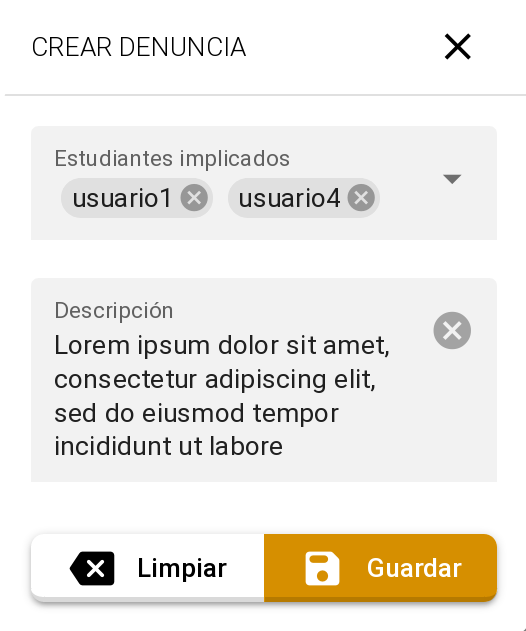
\includegraphics[width=0.5\textwidth]{images/prototypes/cdis-create-denuncia-capture.png} }
\end{userstory}

% Para crear un caso disciplinario basta con asignar una comisi�n a una denuncia pendiente:
% \begin{userstory}
% 	\storyname{ Crear caso disciplinario }
% 	\storyuser{ Decano }
% 	\storyiter{ 1 }
% 	\storypriority{ Alta }
% 	\storyrisk{ Medio }
% 	\storypoints{ 0.4 }
% 	\storyprogrammer{ \authorA }
% 	\storydescription{ Como Decano quiero crear caso disciplinario. }
% 	\storyobservation{ }
% 	\storyinterface{ 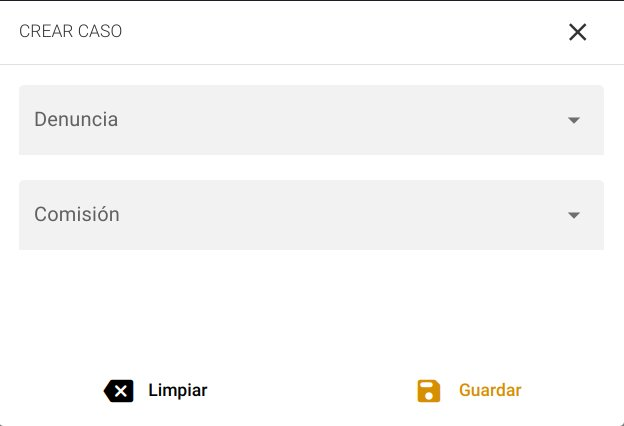
\includegraphics[width=0.5\textwidth]{images/prototypes/cdis-create-caso.png} }
% \end{userstory}